\documentclass[b5paper]{standalone}
\usepackage{fontspec}
\usepackage{polyglossia}
\usepackage{tikz}
\usepackage{ifthen}   
\usepackage{amsmath}
\usetikzlibrary{calc}
%
\setmainlanguage{english}
\setotherlanguages{arabic}
\newfontfamily\arabicfont[Scale=1.0,Script=Arabic]{Scheherazade}
\newfontfamily\urdufont[Scale=1.0,Script=Arabic]{XB Tabriz}

\begin{document}
\begin{urdufont}
\begin{tikzpicture}
%
%right figure
\begin{scope}[xshift=6cm]
%grid
%\draw[gray,thick] (-2,-2) grid (2,2);
%\draw[gray,thin,xstep=0.1,ystep=0.1] (-2,-2) grid (2,2);
%arrow heads
\draw[->] (0.4,0.46)--++(45:0.001);
\draw[->] (0.3,0.66)--++(200:0.001);
\draw[->] (-0.55,-0.7)--++(10:0.001);
%axis
\draw[gray] (0,1.2)node[left]{$B$}--(0,-1.2);
\draw [gray](-1.2,0)--(1.2,0)node [right]{$H$} ;
\draw(0.8,-1) node{ب};
%BH curve
\node[inner sep=0] at (0,0) {
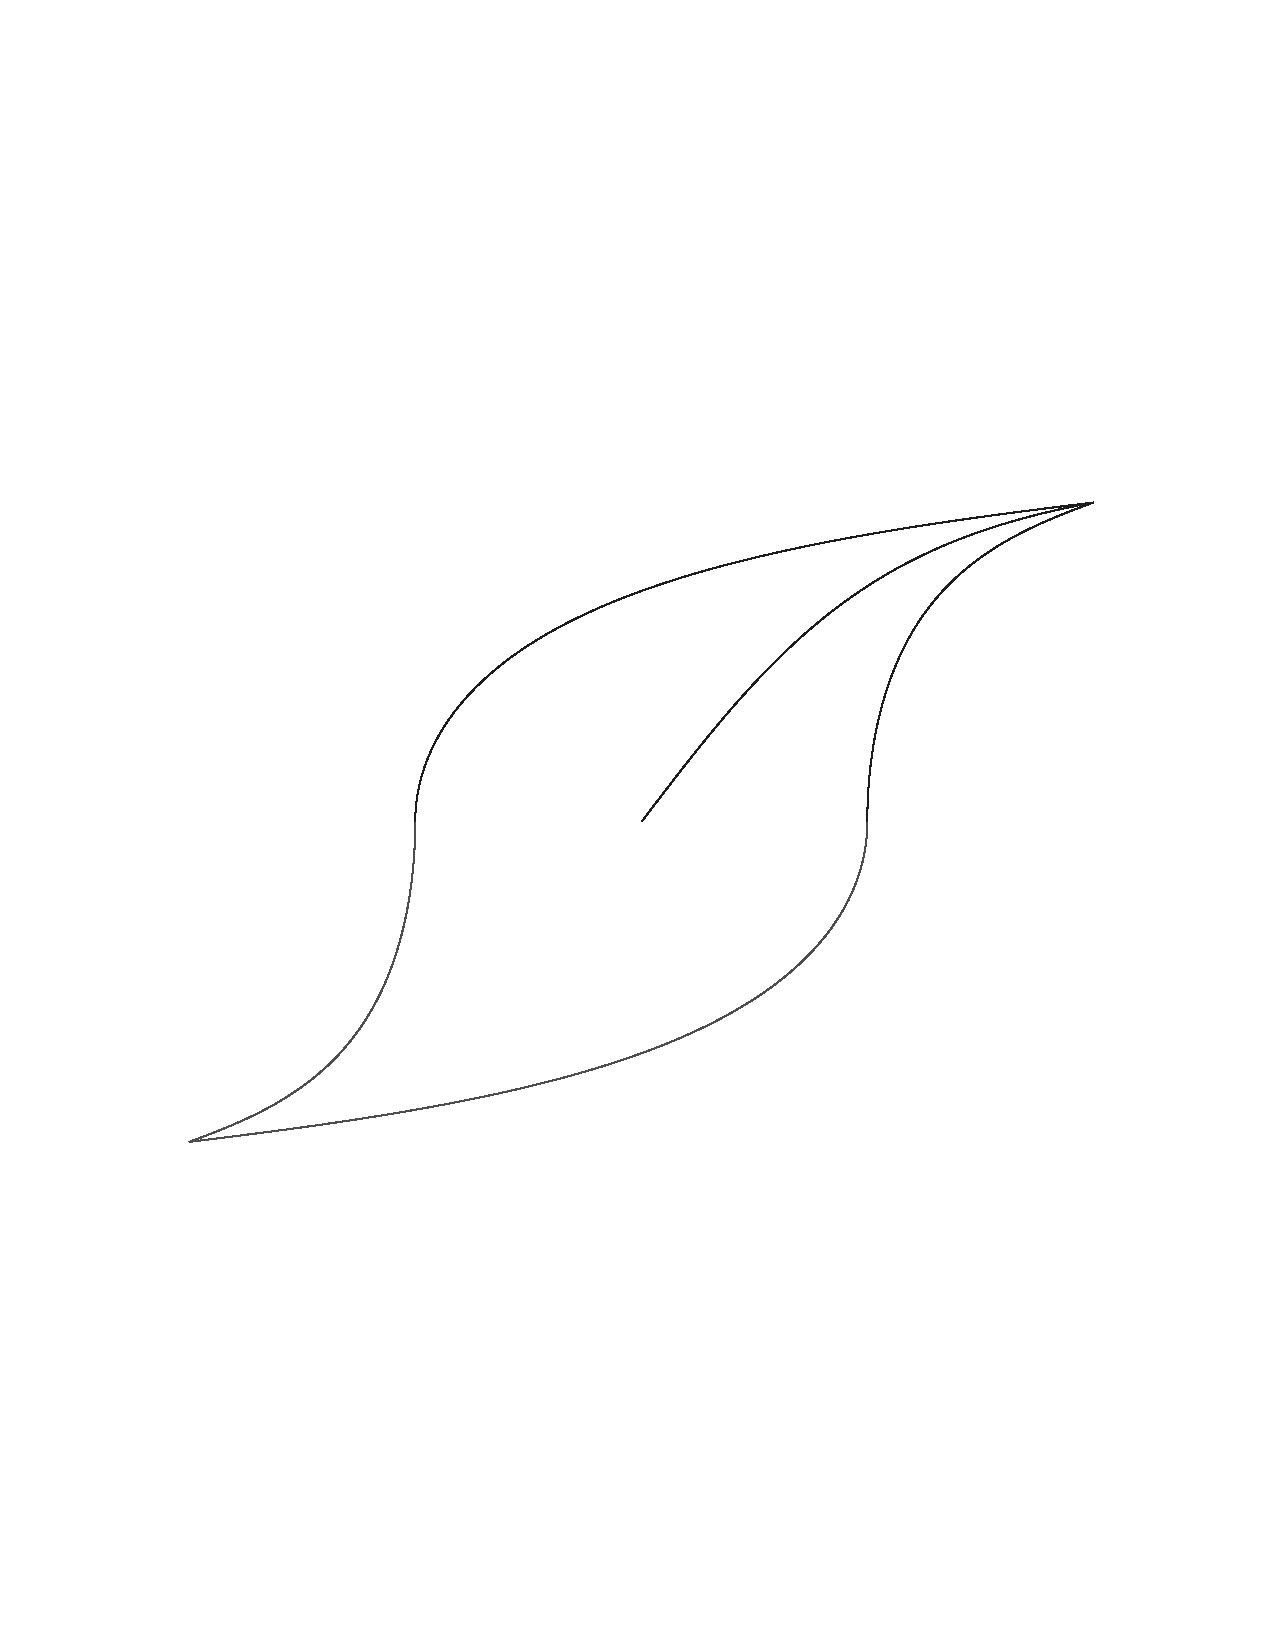
\includegraphics[width=.25\textwidth]{BHhysterisysSingleLoop}
};
%a,b,c,d,e
\draw (0,0) node[below]{$a$};
\draw (1.2,0.8) node[right]{$b$};
\draw (-0.2,0.7) node{$c$};
\draw (-0.7,0.2) node{$d$};
\draw (-1.2,-0.8) node[left]{$e$};
\draw (0.2,-0.75) node{$f$};
\draw (0.7,-0.2) node{$g$};
\end{scope}
%
%--------------------
%left figure
\draw[gray] (0,1.2)node[left]{$B$}--(0,-1.2);
\draw [gray](-1.2,0)--(1.2,0)node [right]{$H$} ;
\draw(0.8,-1) node{الف};
%BH curve
\node[inner sep=0] at (0,0) {
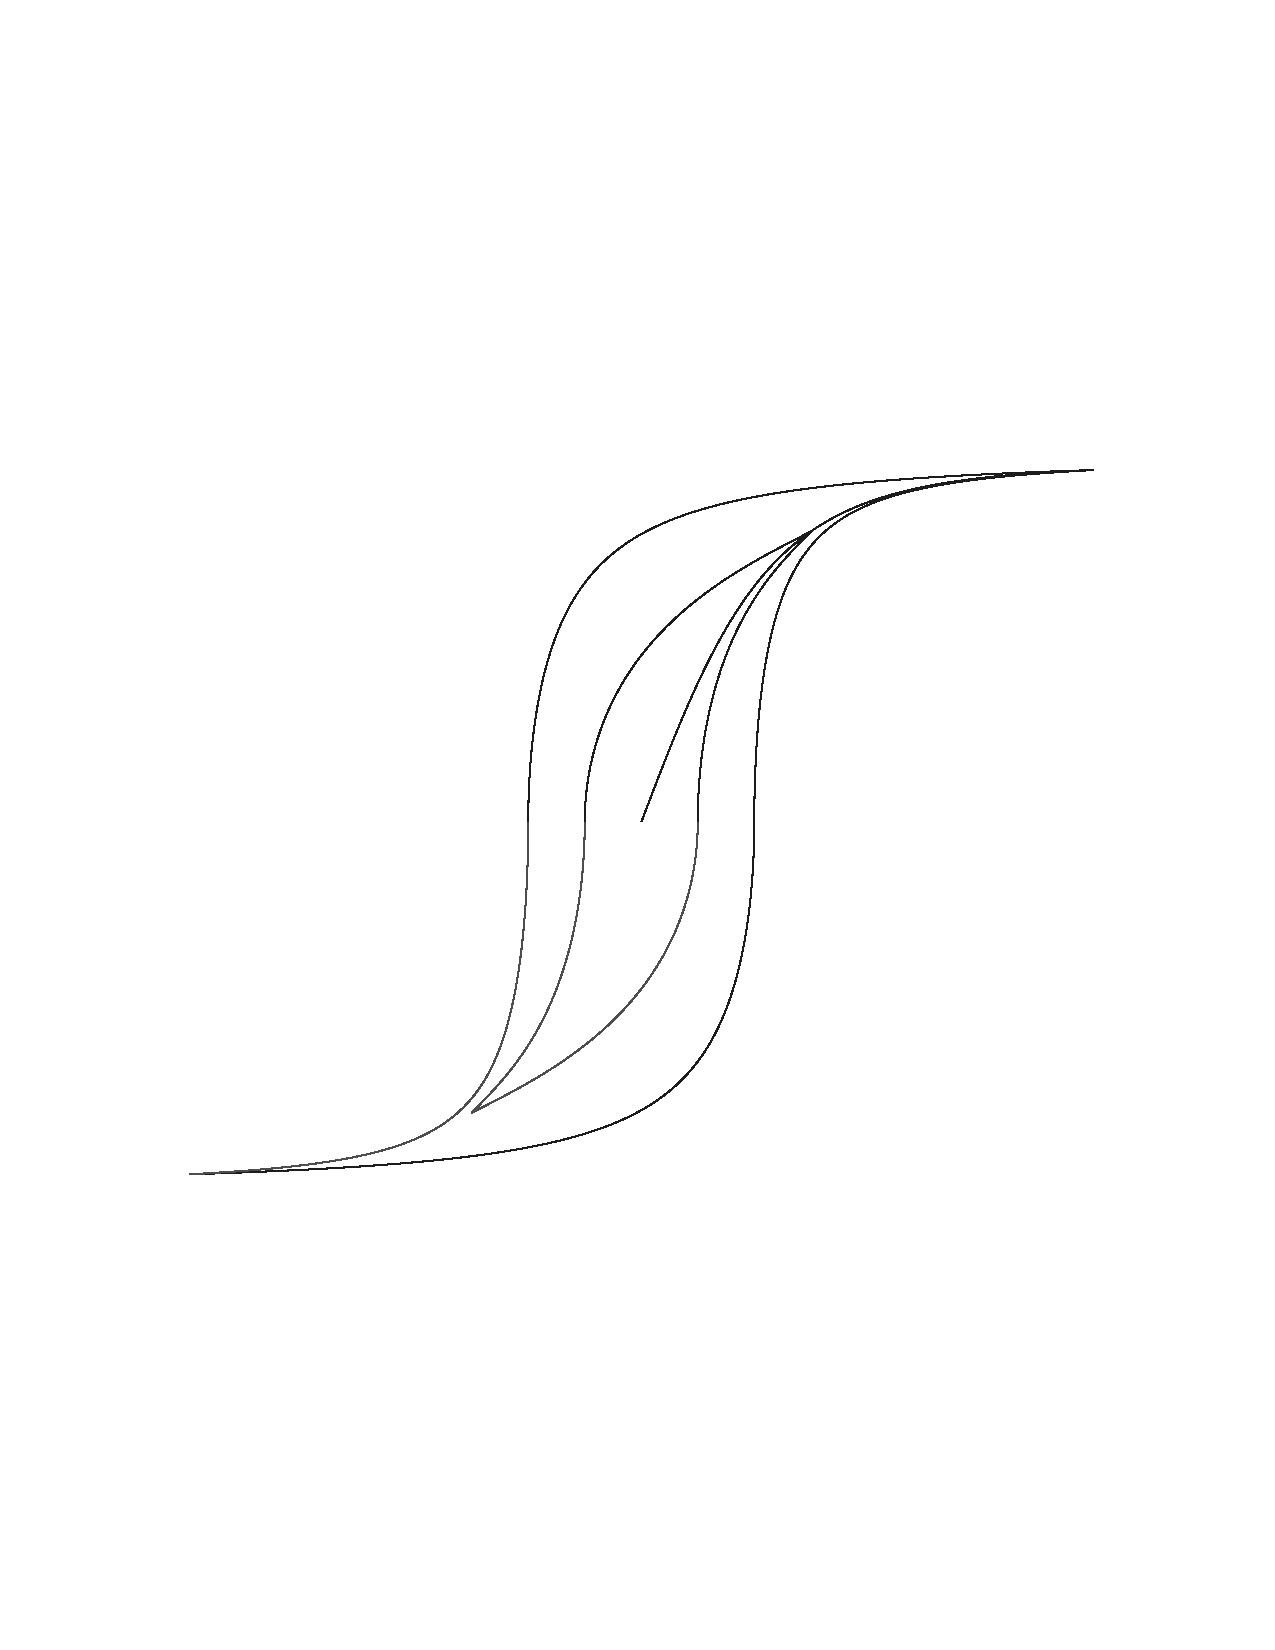
\includegraphics[width=.25\textwidth]{BHhysterisys}
};
\end{tikzpicture}%
\end{urdufont}
\end{document}

